\documentclass[border=2mm]{standalone}
\usepackage{pgfplots}
\pgfplotsset{compat=1.18}
\definecolor{red}{rgb}{0.7, 0.11, 0.11}
\definecolor{blue}{rgb}{0.0, 0.20, 0.42}
\definecolor{green}{rgb}{0.11, 0.35, 0.02}
\begin{document}
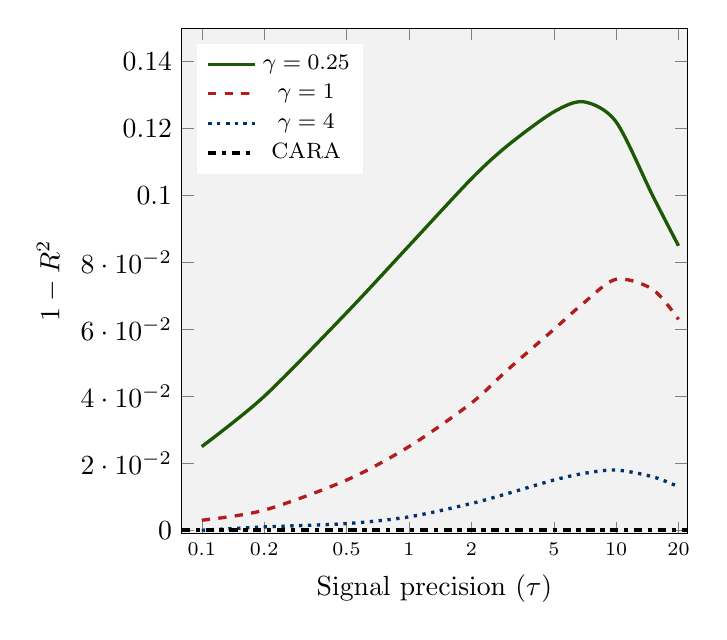
\begin{tikzpicture}
\begin{axis}[
  legend style={draw=none,legend pos=north west,font=\footnotesize},
  ymin=-0.001, ymax=0.15, ylabel={$1-R^2$},
  xmin=0.08, xmax=22, xmode=log,
  xlabel={Signal precision $(\tau)$},
  xtick={0.1,0.2,0.5,1,2,5,10,20},
  xticklabels={0.1,0.2,0.5,1,2,5,10,20},
  xticklabel style={/pgf/number format/1000 sep=,font=\scriptsize},
  width=8cm, height=8cm,
  axis background/.style={fill=black!5}]
\addplot[very thick,color=green,smooth] coordinates {
  (0.1,0.025)(0.2,0.040)(0.5,0.065)(1,0.085)(2,0.105)
  (3,0.115)(5,0.125)(7,0.128)(10,0.122)(15,0.100)(20,0.085)};
\addplot[very thick,color=red,dashed,smooth] coordinates {
  (0.1,0.003)(0.2,0.006)(0.5,0.015)(1,0.025)(2,0.038)
  (3,0.048)(5,0.060)(7,0.068)(10,0.075)(15,0.072)(20,0.063)};
\addplot[very thick,color=blue,dotted,smooth] coordinates {
  (0.1,0.000)(0.2,0.001)(0.5,0.002)(1,0.004)(2,0.008)
  (3,0.011)(5,0.015)(7,0.017)(10,0.018)(15,0.016)(20,0.013)};
\addplot[ultra thick,color=black,dashdotted] coordinates {(0.08,0)(22,0)};
\legend{$\gamma = 0.25$, $\gamma = 1$, $\gamma = 4$, CARA}
\end{axis}
\end{tikzpicture}
\end{document}
